\documentclass{report}
\usepackage{graphicx}
\usepackage{subfigure}
\usepackage{multirow}
\usepackage{wrapfig}
\usepackage{amssymb}
\usepackage{amsmath}
\usepackage{mathrsfs}
\usepackage{enumerate}
% \usepackage{bookmark}

\usepackage{amssymb,amsmath,amsthm,amsfonts}
\usepackage{mathrsfs}
\usepackage{dsfont}
\usepackage{enumerate}

%\newtheorem{mdef}{Definition}
%\newtheorem{theorem}{Theorem}
\newcommand{\eqsplit}[2]{
  \begin{equation}\label{#2}
    \begin{split}
      #1
    \end{split}
  \end{equation}}
\newcommand{\eqnsplit}[1]{
  \begin{eqnarray*}
    #1
  \end{eqnarray*}}
\newcommand{\tran}[1]{
  \tilde{#1}
}
\newcommand{\td}[2]{
  \frac{d #1}{d #2}
}
\newcommand{\pd}[2]{
  \frac{\partial #1}{\partial #2}
}
\newcommand{\ppd}[2]{
  \frac{\partial^2 #1}{\partial #2^2}
}
\newcommand{\pdd}[3]{
  \frac{\partial^2 #1}{\partial #2 \partial #3}
}
\newcommand{\otd}[1]{
  \frac{d}{d #1}
}
\newcommand{\opd}[1]{
  \frac{\partial}{\partial #1}
}
\newcommand{\oppd}[1]{
  \frac{\partial^2}{\partial #1^2}
}
\newcommand{\opdd}[2]{
  \frac{\partial^2}{\partial #1 \partial #2}
}
\newcommand{\ket}[1]{
  |#1\rangle
}
\newcommand{\bra}[1]{
  \langle#1|
}
\newcommand{\inn}[1]{
  \langle#1\rangle
}
\newcommand{\mean}[1]{
  \langle#1\rangle
}
\newcommand{\tr}{
  \text{tr}\,
}
\newcommand{\re}{
  \text{Re}\,
}
\newcommand\im{
  \text{Im}\,
}
\newcommand{\var}{
  \text{var}
}
\newcommand{\arcsinh}{
  \sinh^{-1}
}
\newcommand{\arccosh}{
  \cosh^{-1}
}
\newcommand{\erfc}{
  \text{erfc}
}
\newcommand{\E}{
  \mathbb{E}
}
\renewcommand{\P}{
  \mathbb{P}
}
\newcommand{\I}[1]{
  \mathbf{1}_{\{#1\}}
}
\newcommand{\1}[1]{
  \mathds{1}_{\{#1\}}
}
\newcommand{\diag}{
  \text{diag\,}
}
\newcommand{\M}{
  {\text{max}}
}
\newcommand{\m}{
  {\text{min}}
}
\newcommand{\ph}{
  {\text{arg}\,}
}
\newcommand\erf{
  \text{erf}
}
\renewcommand\vec[1]{
  \mathbf{#1}
}
\newcommand\mtx[1]{
  \mathbf{#1}
}
\newcommand\ed{
  \,{\buildrel d \over =}\,
}



\author{Xie Xiaolei}
\date{\today}
\title{Solutions to the Final Term Test}
\begin{document}
\maketitle

\begin{enumerate}[1.]
\item
  \begin{enumerate}[(a)]
  \item We consider the probability
    \begin{eqnarray*}
      && P(X_i < x) \\
      &=& P(\bigcap_{j=1}^k \{Y_{i+j} \le x\}) \\
    \end{eqnarray*}
    Since the $(Y_i)$ are iid with df. $F^{1/k}$, we have
    \begin{eqnarray*}
      && P(\bigcap_{j=1}^k \{Y_{i+j} \le x\}) \\
      &=& [F^{1/k}(x)]^k \\
      &=& F(x) \\
    \end{eqnarray*}
    The distribution function of $X_i$ is $F(x)$.

  \item 
    \begin{proof}
      We want to prove, $\forall n \ge 1, \forall h \ge 1$, $(X_1,
      \cdots, X_n) \ed (X_{1+h}, \cdots, X_{n+h})$.

      When $n = 1$, this is already proven in the solution to the last
      question since $X_i \sim F$, for any $i$.

      Now suppose $(X_1, \cdots, X_n) \ed (X_{1+h}, \cdots, X_{n+h})$
      for some $n \ge 1$ and $\forall h \ge 1$. In the following we
      prove 
      \[
      (X_1, \cdots, X_{n+1}) \ed (X_{1+h}, \cdots, X_{n+1+h})
      \]
      
      In fact we only need to prove the statement for $h=1$. Because
      $(Y_i)$ is an iid sequence, we can always remove the first element
      and relabel the sequence so that the old $Y_{i+1}$ is the new
      $Y_{i}$. Applying the statement for $h=1$ gives $(X_2, \cdots,
      X_{n+1}) \ed (X_{3}, \cdots, X_{n+2})$ with the old indices,
      thus establishing the statement for $h=2$. This procedure can be
      repeated, proving the statement for all $h \geq 1$.

      In the case $h=1$, we need to prove
      \begin{eqnarray*}
        && P(X_1 \le a_1, \cdots, X_{n+1} \le a_{n+1}) \\
        &=& P(X_2 \le a_1, \cdots, X_{n+2} \le a_{n+1})
      \end{eqnarray*}
      We may write
      \begin{eqnarray*}
        && P(X_1 \le a_1, \cdots, X_{n+1} \le a_{n+1}) \\
        &=& P(X_{n+1} \le a_{n+1} | X_1 \le a_1, \cdots, X_{n} \le
        a_{n}) \cdot \\
        && P(X_1 \le a_1, \cdots, X_{n} \le a_{n})
      \end{eqnarray*}
      The conditional probability on the right-hand-side is
      \begin{eqnarray*}
        && P(X_{n+1} \le a_{n+1} | X_1 \le a_1, \cdots, X_{n} \le
        a_{n}) \\
        &=& P(Y_{n+2} \le a_{n+1}, \cdots, Y_{n+k+1} \le a_{n+1} | Y_2
        \le b_1, \cdots, Y_{n+k} \le b_{n+k-1})
      \end{eqnarray*}
      where $b_1, \cdots, b_{n+k-1}$ are constants depending on $a_1,
      \cdots, a_n$. Because $(Y_i)$ are iid, the above conditional
      probability can be factorized
      \begin{eqnarray*}
        && P(Y_{n+2} \le a_{n+1}, \cdots, Y_{n+k+1} \le a_{n+1} | Y_2
        \le b_1, \cdots, Y_{n+k} \le b_{n+k-1}) \\
        &=& P(Y_{n+2} \le a_{n+1} | Y_{n+2} \le b_{n+1}) \cdots
        P(Y_{n+k} \le a_{n+1} | Y_{n+k} \le b_{n+k-1}) \cdot \\
        && P(Y_{n+k+1} \le a_{n+1}) \\
        &=& {F^{1/k}(a_{n+1} \wedge b_{n+1}) \over F^{1/k}(b_{n+1})} \cdots
        {F^{1/k}(a_{n+1} \wedge b_{n+k-1}) \over F^{1/k}(b_{n+k-1})}
        F^{1/k}(a_{n+1})
      \end{eqnarray*}
      
      Analogously,
      \begin{eqnarray*}
        && P(X_2 \le a_1, \cdots, X_{n+2} \le a_{n+1}) \\
        &=& P(X_{n+2} \le a_{n+1} | X_2 \le a_1, \cdots, X_{n+1} \le
        a_{n}) \cdot \\
        && P(X_2 \le a_1, \cdots, X_{n+1} \le a_{n})
      \end{eqnarray*}
      By assumption, $(X_2, \cdots, X_{n+1}) \ed (X_1, \cdots, X_{n})$,
      meaning
      \[
      P(X_2 \le a_1, \cdots, X_{n+1} \le a_{n}) = P(X_1 \le
      a_1, \cdots, X_{n} \le a_{n})
      \]
      It remains to establish
      \begin{eqnarray*}
        && P(X_{n+2} \le a_{n+1} | X_2 \le a_1, \cdots, X_{n+1} \le
        a_{n}) \\
        &=& P(X_{n+1} \le a_{n+1} | X_1 \le a_1, \cdots, X_{n} \le
        a_{n})
      \end{eqnarray*}
      Similar to the calculation before
      \begin{eqnarray*}
        && P(X_{n+2} \le a_{n+1} | X_2 \le a_1, \cdots, X_{n+1} \le
        a_{n})      \\
        &=& P(Y_{n+3} \le a_{n+1}, \cdots, Y_{n+k+2} \le a_{n+1} | Y_3
        \le b_1, \cdots, Y_{n+k+1} \le b_{n+k-1}) \\
        &=& P(Y_{n+3} \le a_{n+1} | Y_{n+3} \le b_{n+1}) \cdots
        P(Y_{n+k+1} \le a_{n+1} | Y_{n+k+1} \le b_{n+k-1}) \cdot \\
        && P(Y_{n+k+2} \le a_{n+1}) \\
        &=& {F^{1/k}(a_{n+1} \wedge b_{n+1}) \over F^{1/k}(b_{n+1})} \cdots
        {F^{1/k}(a_{n+1} \wedge b_{n+k-1}) \over F^{1/k}(b_{n+k-1})}
        F^{1/k}(a_{n+1}) \\
        &=& P(X_{n+2} \le a_{n+1} | X_2 \le a_1, \cdots, X_{n+1} \le
        a_{n})\\
      \end{eqnarray*}
      So we may conclude
      \begin{eqnarray*}
        P(X_1 \le a_1, \cdots, X_{n+1} \le a_{n+1}) &=& P(X_2 \le a_1,
        \cdots, X_{n+2} \le a_{n+1})
      \end{eqnarray*}
    \end{proof}

  \item Notice that $M_n=\max(X_1, \cdots, X_n) = \max(Y_2, \cdots,
    Y_{n+k})$. Since $(Y_i)$ is an iid sequence
    \[
    P(M_n \le x) = F^{n+k-1 \over k}(x)
    \]
    Because
    \[
    \lim_{n \to \infty} n \bar{F}(u_n) = \tau
    \]
    by Poisson approximation,
    \begin{eqnarray*}
      \lim_{n \to \infty} F^n(u_n) &=& e^{-\tau} \\
      \lim_{n \to \infty} (F^n)^{\frac{n+k-1}{k} \frac{1}{n}} (u_n) &=&
      \lim_{n \to \infty} (e^{-\tau})^{\frac{n+k-1}{k} \frac{1}{n}} =
      e^{-\tau / k} \\
    \end{eqnarray*}
    That is
    \[
    \lim_{n \to \infty} P(M_n \le u_n) = \lim_{n \to \infty} F^{n+k-1 \over k}(u_n) = e^{-\tau / k}
    \]
  \item It is straight-forward to calculate
    \begin{eqnarray*}
      N_n &=& \E \sum_{i=1}^{n-1} I_{\{X_i = X_{i+1}\}} \\
      &=& \sum_{i=1}^{n-1} P(X_i = X_{i+1}) \\
    \end{eqnarray*}
    where
    \begin{eqnarray*}
      && P(X_i = X_{i+1}) \\
      &=& P[Y_{i+1} \ne \max(Y_{i+1}, \cdots,
      Y_{i+k}), Y_{i+k+1} \ne \max(Y_{i+2}, \cdots, Y_{i+k+1})]
    \end{eqnarray*}
    Because $Y_i$ is an iid sequence, the two events of the above
    joint probability are independent. Thus we have
    \begin{eqnarray*}
      P(X_i = X_{i+1}) &=& \left({k-1 \over k}\right)^2
    \end{eqnarray*}
    and
    \begin{eqnarray*}
      N_n &=& (n-1) \left({k-1 \over k}\right)^2 \\
      &\ge& {n-1 \over 4}
    \end{eqnarray*}
    The expected number of equal pairs is at least 1/4 of the number
    of pairs.
  \end{enumerate}

\item
  \begin{enumerate}[(a)]
  \item
    \begin{proof}
      First of all, we show that, if
      \begin{eqnarray}
        \lim_{x \to \infty} \frac{\bar{F}(x - y)}{\bar{F}(x)} &=&
        e^{\gamma y} \label{eq:property}
      \end{eqnarray}
      holds for $y > 0$, it also holds for $y < 0$.
      
      Clearly
      \begin{eqnarray*}
        \lim_{x \to \infty} \frac{\bar{F}(x)}{\bar{F}(x - y)} &=&
        e^{-\gamma y}      
      \end{eqnarray*}
      Because $x - y \to \infty$ as $x \to \infty$, we may replace $x -
      y$ by $x'$ and write
      \begin{eqnarray*}
        \lim_{x \to \infty} \frac{\bar{F}(x' + y)}{\bar{F}(x')} &=&
        e^{-\gamma y}      
      \end{eqnarray*}
      Let $y' = -y < 0$, then we see \eqref{eq:property} also holds for
      $y < 0$.

      Now we assume \eqref{eq:property} holds for all $y \in
      R$. $e_F(u)$ can be easier evaluated by changing the variable of
      integration:
      \begin{eqnarray*}
        e_F(u) &=& \int_{u}^{\infty} \frac{\bar{F}(y)}{\bar{F}(u)} dy
      \end{eqnarray*}
      let $y = \ln z$, so that
      \begin{eqnarray}
        e_F(u) &=& \int_{e^u}^{\infty} \frac{\bar{F}(\ln
          z)}{\bar{F}(u)}{1 \over z} dz \label{eq:e_F}
      \end{eqnarray}
      Because
      \begin{eqnarray*}
        \lim_{x \to \infty} {\bar{F}(x - y) \over \bar{F}(x)} &=&
        e^{\gamma y}
      \end{eqnarray*}
      $\bar{F}(\ln x)$ is a regularly varying function with index
      $-\gamma$:
      \begin{eqnarray*}
        \lim_{x \to \infty} {\bar{F}(\ln(a x)) \over \bar{F}(\ln(x))}
        &=& \lim_{x \to \infty} {\bar{F}(\ln x + \ln a) \over
          \bar{F}(\ln x)} \\
        &=& e^{-\gamma \ln a} \\
        &=& a^{-\gamma}
      \end{eqnarray*}
      where the second last equality is due to \eqref{eq:property}.

      Now that $\bar{F}(\ln x)$ is regularly varying, we may write
      $\bar{F}(\ln x) = L(x) x^{-\gamma}$ as $x \to \infty$, where
      $L(x)$ is a slowing varying function. Inserting this
      representation into \eqref{eq:e_F} and applying Karamata's
      theorem, we obtain
      \begin{eqnarray*}
        \lim_{u \to \infty} e_F(u) &=& \lim_{u \to \infty}
        \int_{e^u}^{\infty} {L(z) z^{-\gamma - 1} \over L(e^u)
          e^{-\gamma u}} dz \\
        &=& \lim_{u \to \infty} {1 \over
          \gamma} L(e^u) e^{-\gamma u} [L(e^u) e^{-\gamma u}]^{-1} \\
        &=& {1 \over \gamma}
      \end{eqnarray*}
      
      % Let $y = \ln y' + u$. Then we have
      % \begin{eqnarray*}
      %   e_F(u) &=& \int_{1}^{\infty} \frac{\bar{F}(\ln y' +
      %     u)}{\bar{F}(u)}{1 \over y'} dy' \\
      % \end{eqnarray*}
      % Applying \eqref{eq:property} to the integrand gives
      % \begin{eqnarray*}
      %   \lim_{u \to \infty} e_F(u) &=& \lim_{u \to \infty}
      %   \int_{1}^{\infty} \frac{\bar{F}(\ln y' + u)}{\bar{F}(u)}{1 \over
      %     y'} dy' \\
      %   &=& \int_{1}^{\infty} e^{-\gamma \ln y'}{1 \over
      %     y'} dy' \\
      %   &=& \int_{1}^{\infty} {1 \over y'^{\gamma + 1}} dy' \\
      % \end{eqnarray*}
      % By Karamata's theorem we have
      % \begin{eqnarray*}
      %   \lim_{u \to \infty} e_F(u) &=& - {1 \over \gamma} \left[{1 \over
      %       y'^\gamma}\right]_{y'=1}^{\infty} = {1 \over \gamma}\\
      % \end{eqnarray*}
    \end{proof}
    % \begin{eqnarray*}
    %   e_F(u) &=& \int_{u}^{\infty} {\bar{F}(y) \over \bar{F}(u)} dy
    % \end{eqnarray*}
    % Let $y = \ln z + u$ and change the variable of integration to
    % $z$. We get
    % \begin{eqnarray*}
    %   e_F(u) &=& \int_{1}^{\infty} {\bar{F}(\ln z + ) \over \bar{F}(u)} dz
    % \end{eqnarray*}
    % Due to the assumed property we have
    % \begin{eqnarray*}
    %   \lim_{z \to \infty} {\bar{F}(u+z) \over \bar{F}(u)} &=&
    %   e^{-\gamma z}
    % \end{eqnarray*}
    % So
    % \begin{eqnarray*}
    %   \lim_{u \to \infty} e_F(u) &=& \int_{0}^{\infty} e^{-\gamma z}
    %   dz \\
    %   &=& {1 \over \gamma}
    % \end{eqnarray*}

  \item
    \begin{enumerate}[(i)]
    \item Since $\bar{F}$ is regularly varying, it is an
      subexponential function, implying
      \[
      \lim_{x \to \infty} {\bar{F}(x - y) \over \bar{F}(x)} = 1
      \]
      according to lemma 1.3.5 of EKM. This means $\gamma =
      0$. Then it follows $\lim_{u \to \infty} e(u) = \infty$.

    \item For $\text{Exp}(\lambda)$, $\bar{F}(x) = \lambda e^{-\lambda
        x}$, hence
      \begin{eqnarray*}
        \lim_{x \to \infty} {\bar{F}(x - y) \over \bar{F}(x)} &=&
        e^{-\lambda (x - y + x)} \\
        &=& e^{\lambda y}
      \end{eqnarray*}
      So it follows $\lim_{u \to \infty} e_F(u) = 1/\lambda$.

    \item When $F$ is standard normal,
      \begin{eqnarray*}
        \lim_{x \to \infty} {\bar{F}(x - y) \over \bar{F}(x)} &=&
        \lim_{x \to \infty} \frac{
          \int_{x-y}^{\infty} e^{z^2/2} {dz \over \sqrt{2\pi}}
        }{
          \int_{x}^{\infty} e^{z^2/2} {dz \over \sqrt{2\pi}}
        }
      \end{eqnarray*}
      Applying l'Hopital's rule, we have
      \begin{eqnarray*}
        \lim_{x \to \infty} {\bar{F}(x - y) \over \bar{F}(x)} &=&
        \lim_{x \to \infty} {e^{-(x-y)^2/2} \over e^{-x^2/2}} = \infty\\
      \end{eqnarray*}
      That is, $\gamma = \infty$ and $\lim_{u \to \infty} e_F(u) =
      0$.
    \end{enumerate}
  \end{enumerate}
\item
  \begin{enumerate}{(a)}
    \begin{enumerate}[(i)]
    \item The Cauchy distribution has regularly varying tail with index
      -1, which we prove below, hence it belongs to
      $\text{MDA}(\Phi_{1})$.

      \begin{proof}
        \begin{eqnarray*}
          \lim_{x \to \infty} {\bar{F}(ax) \over \bar{F}(x)} &=&
          \lim_{x \to \infty}
          {
            1/2 - {1 \over \pi} \arctan(ax)
            \over
            1/2 - {1 \over \pi} \arctan(x)
          }
        \end{eqnarray*}
        Using l'Hopital's rule, we have
        \begin{eqnarray*}
          \lim_{x \to \infty}
          {
            1/2 - {1 \over \pi} \arctan(ax)
            \over
            1/2 - {1 \over \pi} \arctan(x)
          } &=&
          \lim_{x \to \infty} {
            a(x^2 + 1)
            \over
            a^2 x^2 + 1
          } = {1 \over a}
        \end{eqnarray*}
      \end{proof}

    \item For a simulated sample of size 1000, the Hill and the
      Pickands, Dekkers-Einmahl plots are shown in figure
      \ref{fig:Hill-Pickands-1000}.
      \begin{figure}[htb!]
        \centering
        \subfigure[sample size 1000, $\var(\xi^{(H)})$ = 0.0102, $\var(\xi^{(P)})$ = 2.5723]{
          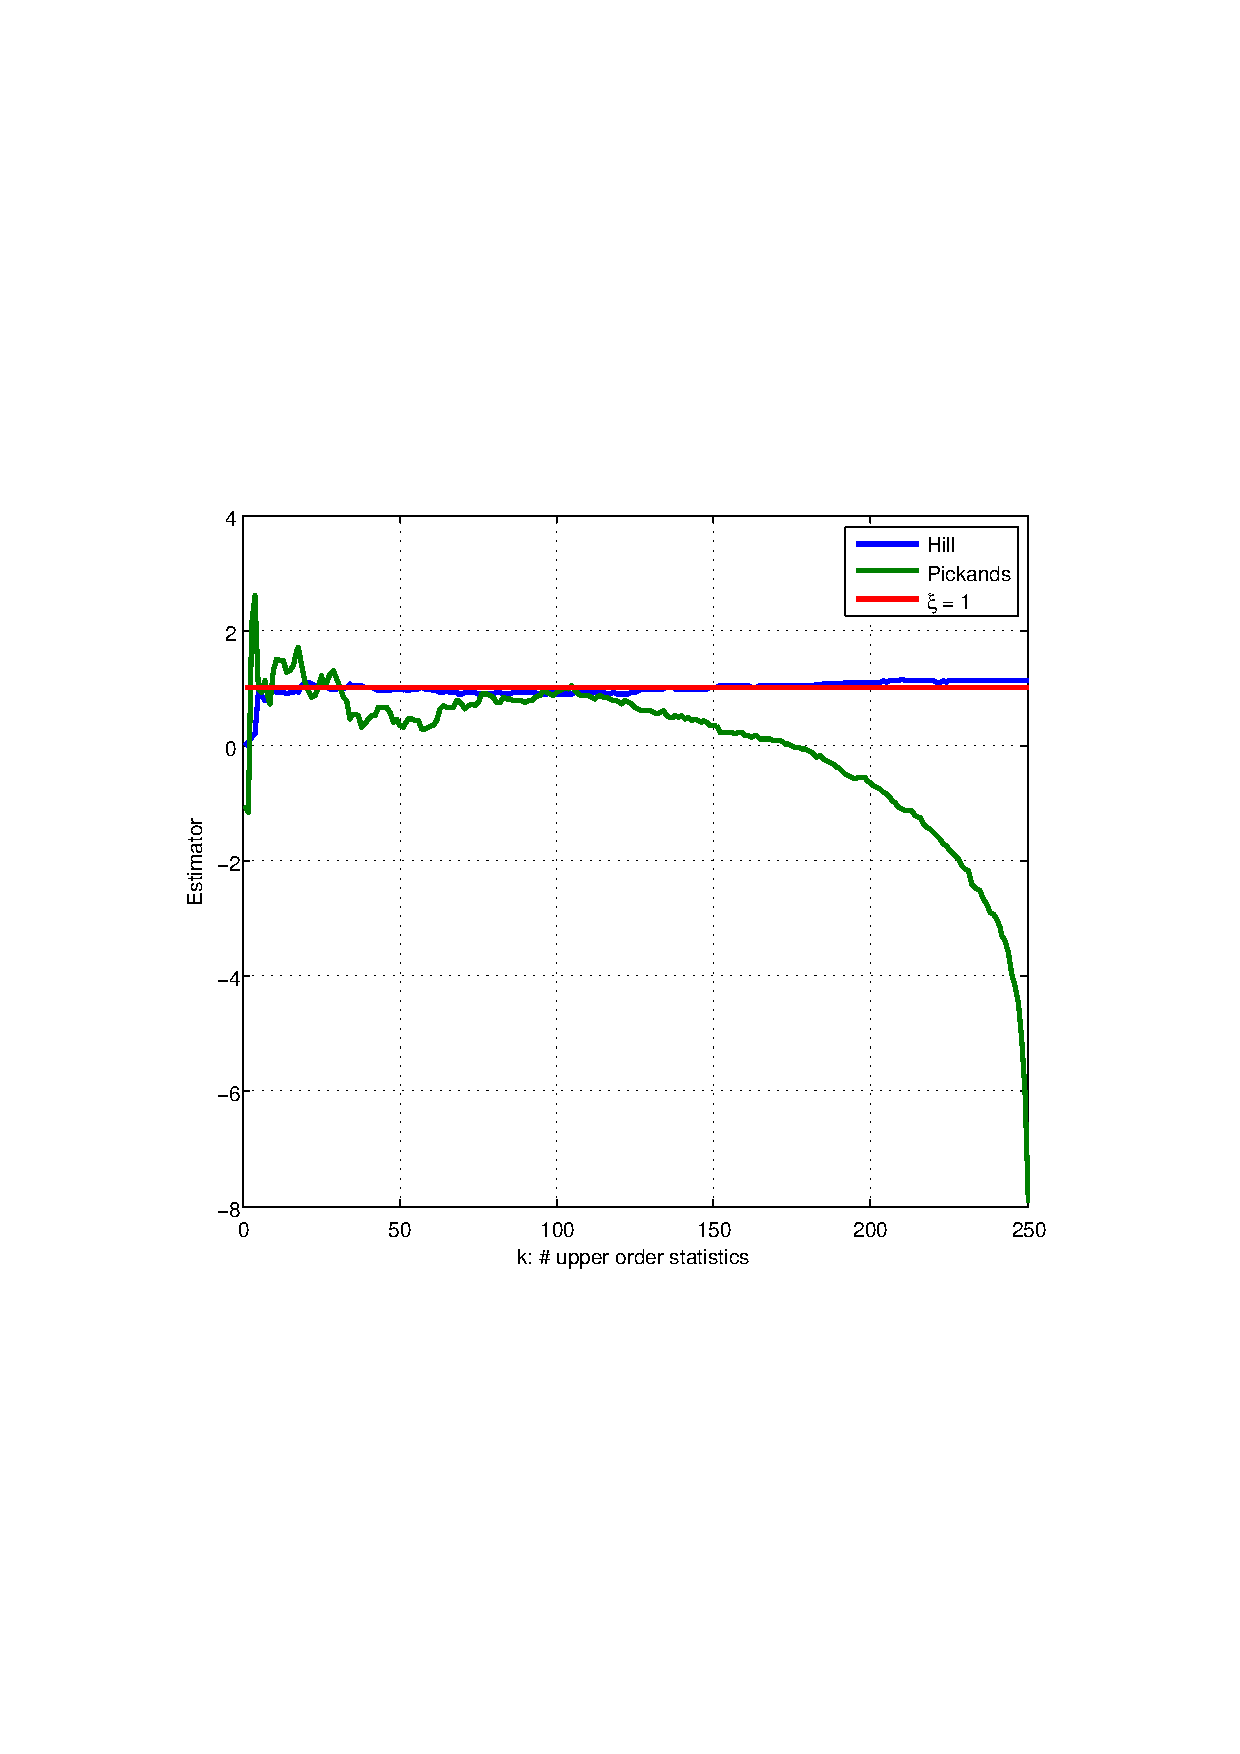
\includegraphics[scale=0.35, clip=true, trim=74 232 94 186]{Hill-Pickands-1000.pdf}
          \label{fig:Hill-Pickands-1000}
        }
        \subfigure[sample size 100, $\var(\xi^{(H)})$ = 0.1019, $\var(\xi^{(P)})$ = 2.8868]{
          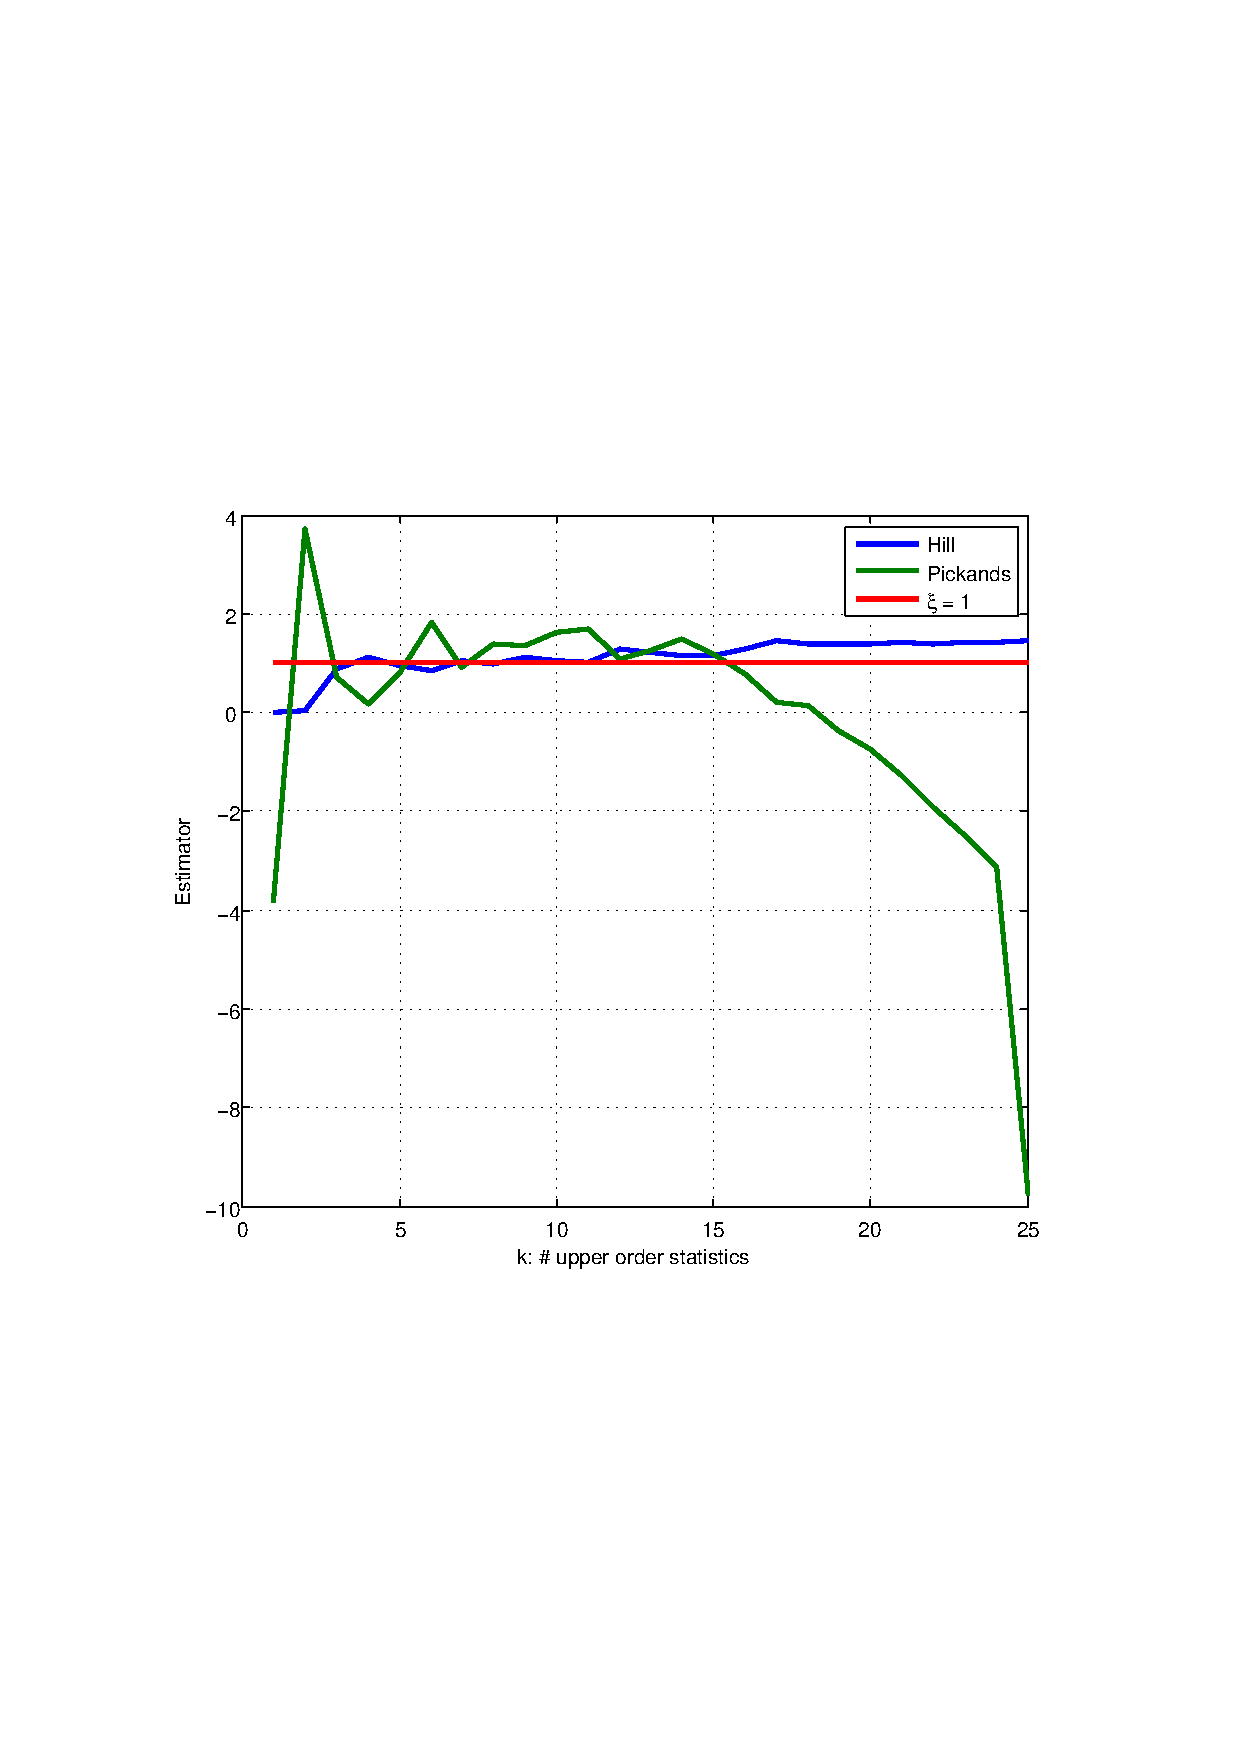
\includegraphics[scale=0.35, clip=true, trim=86 232 94 186]{Hill-Pickands-100.pdf}
          \label{fig:Hill-Pickands-100}
        }
        \caption{\small \it: Hill and Pickands estimator of the extreme
          value index $\xi$.}
        \label{fig:Hill-Pickands}
      \end{figure}
      Clearly, when the sample size is significantly smaller, both
      estimators have larger variances.
    \end{enumerate}

  \item
  \item 
    \begin{enumerate}[(i)]
    \item The Hill plot showing the tail indices of the gains,
      losses, and absolute values of the log-returns are shown in
      figure \ref{fig:Hill-TailIndices}.
      \begin{figure}[htb!]
        \centering
        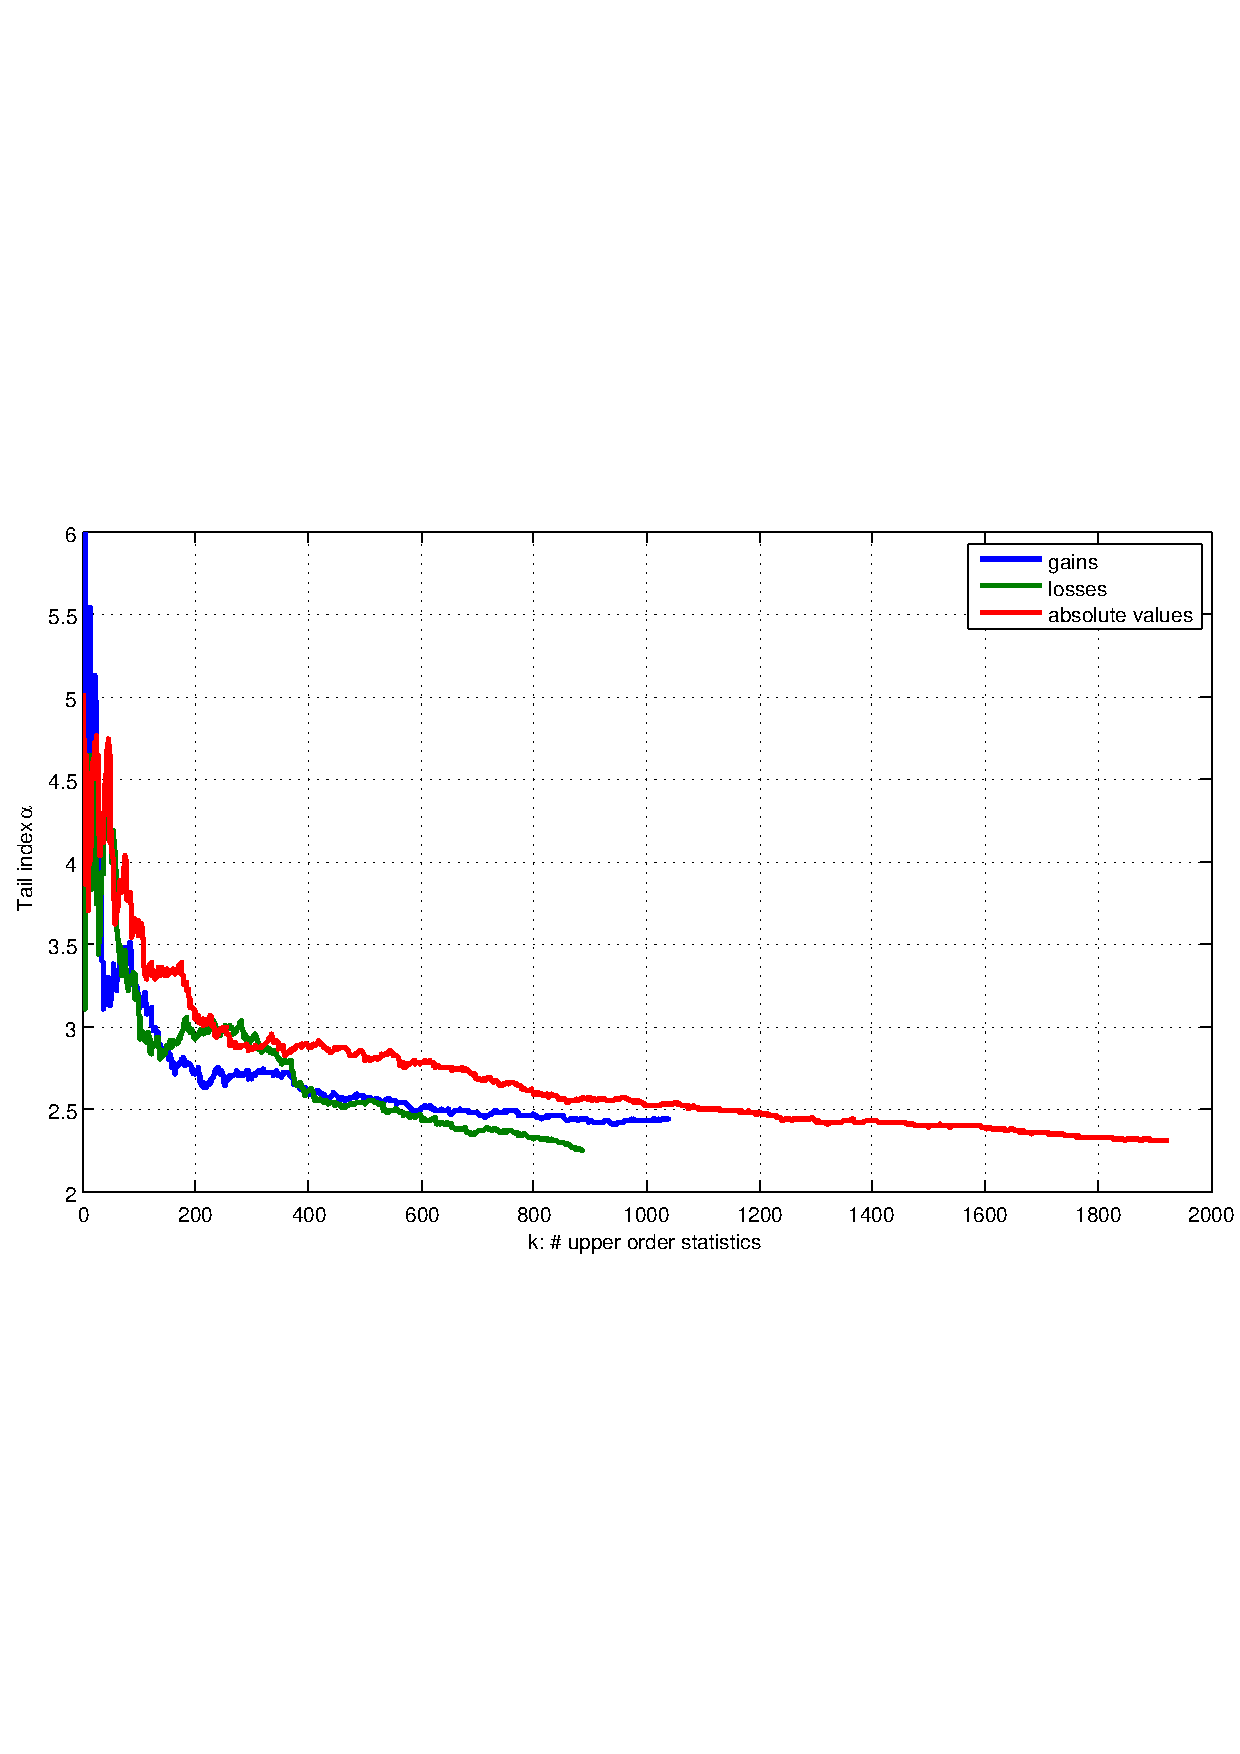
\includegraphics[scale=0.6, clip=true, trim=0 240 0
        194]{Hill-TailIndices.pdf}
        \caption{\small \it: Hill plot of the tail indices $\xi$.}
        \label{fig:Hill-TailIndices}
      \end{figure}
      
    \item Reasonable estimates of the 3 tail indices are listed in
      table \ref{tab:SP500_tail_indices}.
      \begin{table}[htb!]
        \centering
        \begin{tabular}{c|c|c|c}
          & k & tail index & sample size\\
          \hline
          Gains & 289 & 2.72 & 10389\\
          \hline
          Losses & 232 & 3.00 & 8871\\
          \hline
          Absolute values & 287 & 2.89 & 19260\\
        \end{tabular}
        \caption{Tail indices of the S\&P 500 index}
        \label{tab:SP500_tail_indices}
      \end{table}

    \item Using Hill's method, $C$ is estimated as
      \[
      \hat{C} = {k \over n} X_{k, n}^{\hat{\alpha}^{(H)}}
      \]
      where $X_{k,n}$ is the k-th upper order statistic of $X$. Using
      this method, the 99\% quantile as a function of k is plotted in
      figure \ref{fig:99_percentile}.
      \begin{figure}[htb!]
        \centering
        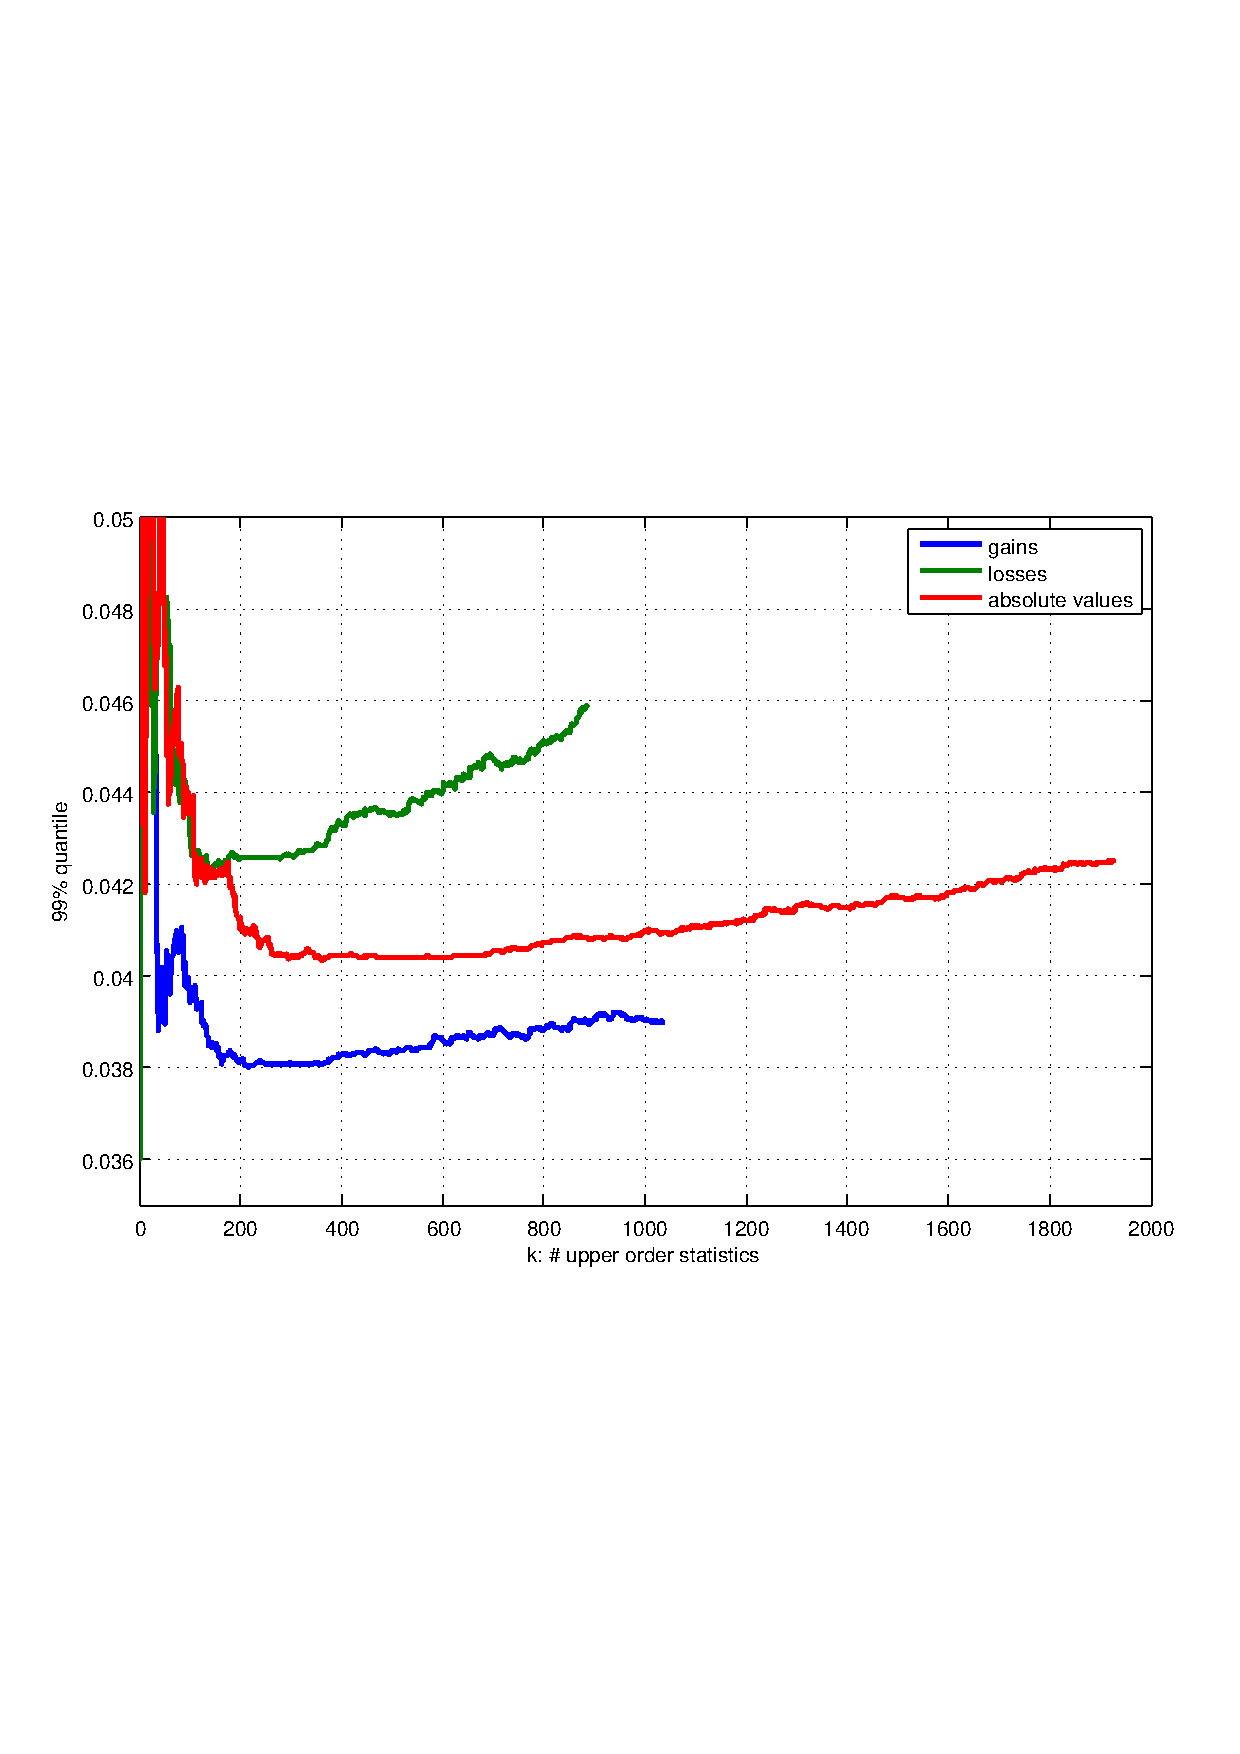
\includegraphics[scale=0.6, clip=true, trim=20 233 28
        185]{99_percentile.pdf}
        \caption{\small \it: 99\% quantile of gains, losses and the
          absolute returns.}
        \label{fig:99_percentile}
      \end{figure}

      Figure \ref{fig:99_percentile} shows the gains have
      significantly lower values for the 99\% quantile than do the
      losses. Hence it confirms that losses 
      indeed have heavier tails than do gains. Around $k=285$, the
      quantile estimates are stable. So $k=285$ is recommended.
    \end{enumerate}
  \end{enumerate}
\end{enumerate}
\end{document}
